\begin{frame}
\begin{table}
\centering
\caption{Wyniki dla zestawu danych SolomonPotvinBengio}
\begin{tabular}{c|c|c}
zestaw & najlepszy opublikowany & najlepszy znaleziony \\ \hline
$rc\_205.1 (n=14)$ & $(0, 343.21)$ & $(0, 343.21)$ \\
$rc\_203.4 (n=15)$ & $(0, 314.29)$ & $(0, 314.29)$ \\
$rc\_203.1 (n=19)$ & $(0, 453.48)$ & $(0, 479.83)$ \\
$rc\_201.1 (n=20)$ & $(0, 444.54)$ & $(0, 444.54)$ \\
$rc\_201.2 (n=26)$ & $(0, 711.54)$ & $(1, 737.38)$ \\
$rc\_201.3 (n=32)$ & $(0, 790.61)$ & $(2, 809.72)$ \\
$rc\_204.1 (n=46)$ & $(0, 878.64)$ & $(4, 990.07)$ 
\end{tabular}
\end{table}
\end{frame}

\begin{frame}
    \begin{figure}
        \centering
        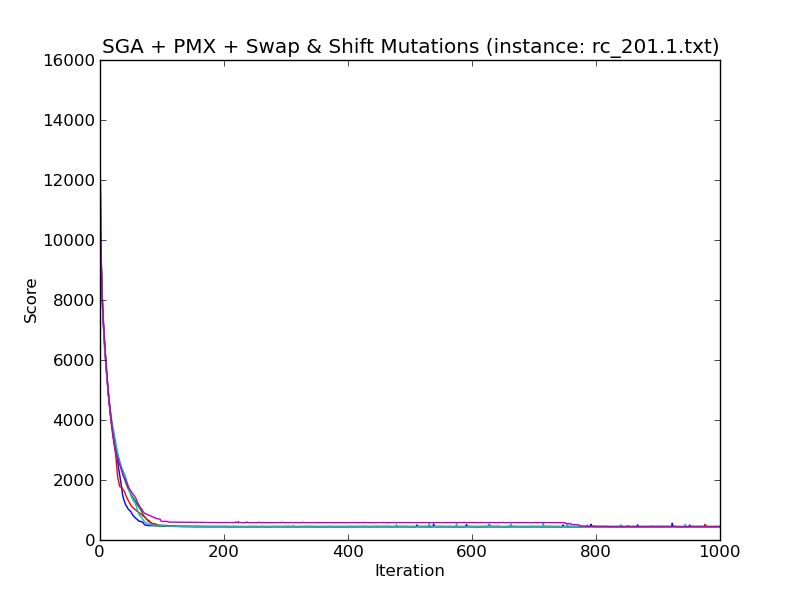
\includegraphics[width=10cm]{charts/rc_201_1.png}
        \caption{rc\_201.1 (n=20)}
    \end{figure}
\end{frame}

\begin{frame}
    \begin{figure}
        \centering
        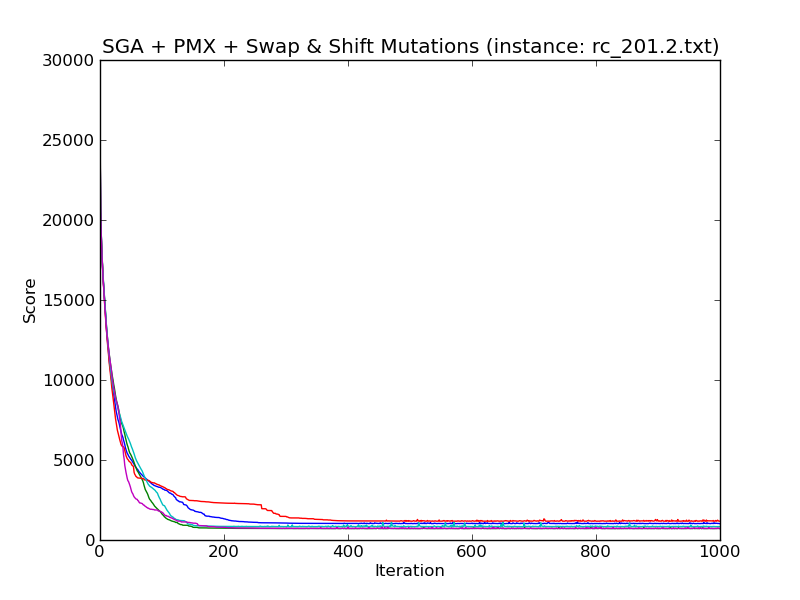
\includegraphics[width=10cm]{charts/rc_201_2.png}
        \caption{rc\_201.2 (n=26)}
    \end{figure}
\end{frame}

\begin{frame}
    \begin{figure}
        \centering
        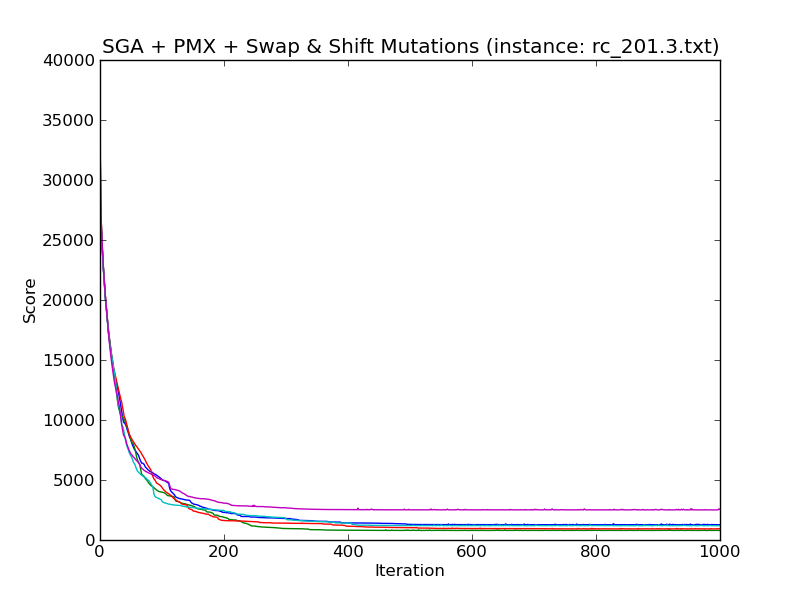
\includegraphics[width=10cm]{charts/rc_201_3.png}
        \caption{rc\_201.3 (n=32)}
    \end{figure}
\end{frame}

\begin{frame}
    \begin{figure}
        \centering
        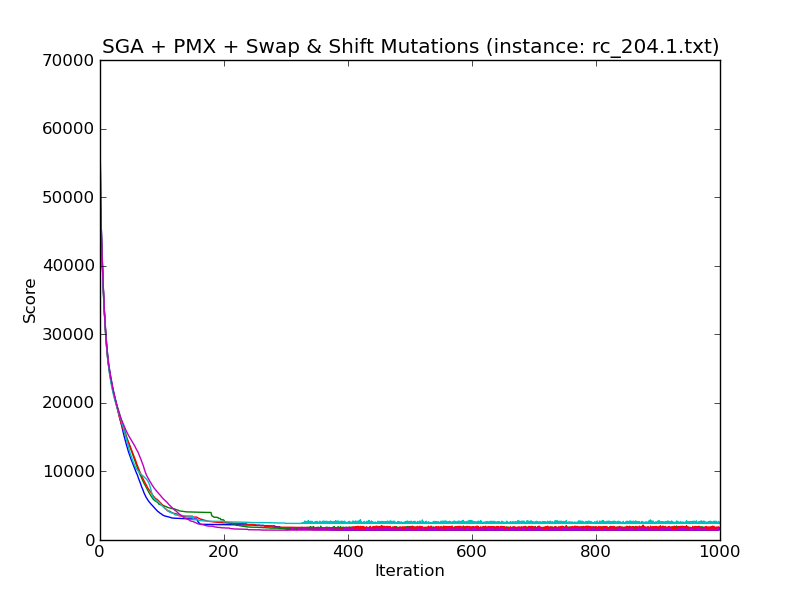
\includegraphics[width=10cm]{charts/rc_204_1.png}
        \caption{rc\_204.1 (n=46)}       
    \end{figure}
\end{frame}

